\documentclass[a4paper, table]{article}

\usepackage{xcolor}
\usepackage{amssymb} 
\usepackage[a4paper]{geometry}
\usepackage[T1]{fontenc}
\usepackage[utf8]{inputenc}
\usepackage{graphicx}
\graphicspath{ {images/} }
\usepackage{todonotes}
\usepackage{hyperref}
\hypersetup{
    colorlinks=true,
    linkcolor=black,
    filecolor=magenta,
    urlcolor=blue
}
% changes font
\usepackage[style=verbose-ibid,backend=bibtex]{biblatex}
\bibliography{wipro-main-doc}

\newcommand{\tabitem}{~~\llap{\textbullet}~~}

\usepackage{times}

% Set name of image label
\renewcommand{\figurename}{Abbildung}

\title{
    {Wirtschaftsprojekt} \\
    \vspace{10mm}
    { Herbstsemester 2022 } \\
    \vspace{10mm}
    % https://commons.wikimedia.org/wiki/File:HSLU_2022_logo.svg
    {
\includegraphics[width=75mm]{img/hsluLogo2022.png}}
}

\author{Yannis Kr\"amer und Nicolas Wiedmer}
% TODO: Update date
\date{22.09.2022}

\begin{document}

\maketitle

\newpage

\noindent
\fontsize{12}{14}
\textbf{Wirtschaftsprojekt an der Hochschule Luzern -- Informatik} \\ \vspace*{0.6cm}

\fontsize{10.95}{12}
\noindent
\textbf{Titel:} STAIR Discord Bot \\ \vspace*{0.2cm}

\noindent
\textbf{Studentin/Student:} Yannis Kr\"amer \newline \newline
\textbf{Studentin/Student:} Nicolas Wiedmer \newline \newline
\textbf{Studiengang:} BSc Informatik oder Wirtschaftsinformatik  \newline \newline
\textbf{Jahr:} 2022 \newline \newline
\textbf{Betreuungsperson:} Markus Waldmann \newline \newline
\textbf{Expertin/Experte:} \newline \newline
\textbf{Auftraggeberin/Auftraggeber:} STAIR (Martin Steiger \& Estefania Otero)\newline \newline \newline
\textbf{Codierung / Klassifizierung der Arbeit:}\\
$\boxtimes$ \"Offentlich 
$\square$ Vertraulich


%%% you can use \boxtimes for filling a cross inside the square
%%% e.g., $\boxtimes$ A: Einsicht 	(Normalfall) 


\paragraph{\textbf{Eidesstattliche Erkl\"arung}}
Ich erkl\"are hiermit, dass ich/wir die vorliegende Arbeit selbst\"andig und ohne unerlaubte fremde Hilfe angefertigt haben, alle verwendeten Quellen, Literatur und andere Hilfsmittel angegeben haben, w\"ortlich oder inhaltlich entnommene Stellen als solche kenntlich gemacht haben, das Vertraulichkeitsinteresse des Auftraggebers wahren und die Urheberrechtsbestimmungen der Hochschule Luzern respektieren werden. \newline \newline
Ort / Datum, Unterschrift	\underline{\hspace*{8cm}} \newline \newline
Ort / Datum, Unterschrift	\underline{\hspace*{8cm}} \newline \newline \newline
\textbf{Ausschliesslich bei Abgabe in gedruckter Form: \\
Eingangsvisum durch das Sekretariat auszuf\"ullen}\newline \newline
Rotkreuz, den	\underline{\hspace*{4cm}}	\hspace*{1cm} Visum:	\underline{\hspace*{4cm}}

\newpage
\section*{I{\hspace*{1cm}}Abstract}
\todo{schreiben}

\newpage

\tableofcontents
\newpage
\section{Problem, Fragestellung, Vision}

\todo{Yannis schreiben}

\section{Stand der Technik}

\subsection{Sprach- und Text-Messenger}

\subsection{Discord}
Der Online Dienst Discord ist ein Instant-Messaging und Chat Tool mit Sprach- und Videokonferenz Funktion. 
Er kann online auf einer Webseite, oder mit Hilfe eines Clients lokal aufgerufen werden. 
Discord ist für alle g\"angigen Betriebssysteme verfügbar und unterstützt zudem die Benützung auf mobilen Endger\"aten.

\subsubsection{Geschichte}
Urspr\"unglich wurde Discord f\"ur Computerspiele geschaffen, um die Kommuniaktion zwischen den Spielkameraden zu vereinfachen/
verbessern. Das Ziel war es, nebst der komplexen Spielmechanik einen Messanger zu bauen, der sich als
benutzerfreundlich und effizient erweist. Das Unternehmen Discord Inc (damals noch Hammer \& Chisel) wurde im Jahr 2012
als Start Up gegr\"undet.\autocite{noauthor_discord_2021} Im Jahre 2014 konnte die Unternehmung Hammer \& Chisel f\"ur die Weiterentwicklung Ihrer
Applikation auf zus\"atzliche Finanzierungsmittel, von anderen Unternehmen zur Verfügung gestellt, zurückgreifen.

2015 folgte die Veröffentlichung unter der Domain "discordapp.com". Der Sprach- und Messanger Dienstleister erfreute sich schnell
grosser Beliebtheit und geriet so in das Blickfeld grösserer Investoren wie z.B. Warner Media, die den Dienst 2016 mit rund 
20 Millionen US-Dollar unterstützte. \autocite{noauthor_warner_2022} .
2018 k\"undete auch Microsoft Discord Unterst\"utzung f\"ur ihre XBox Live Nutzer an und unterst\"utzte Discord mit einer Finanzierung
von 150 Millionen US-Dollar. Bewertet wurde Discord Inc nun auf etwa 2 Milliarden US-Dollar.

Aufgrund der Covid-19 Pandemie und den steigenden Benutzerzahlen stellte sich Discord auch f\"ur andere Zielgruppen ein. 
So wurde der Fokus von Videospielen weggelenkt auf einen universellen Kommunikations-und Chat Client, um es f\"ur andere Branchen, 
wie das Schulwesen oder innerhalb Unternehmen, ansprechender zu machen. Damit \"anderte das Unternehmen ihr Motto 
von \textit{Chat for Gamers} zu \textit{Chat for Communities and Friends} und f\"uhrte Servervorlagen ein.

Heute hat Discord mehr als 140 Millionen monatlich aktive User, verwaltet etwa 13.5 Millionen aktive Server und
wird auf 15 Milliarden US-Dollar gewertet. (Stand 2021) \autocite{david_curry_discord_2022}

\autocite{noauthor_discord_2022}


\subsubsection{Discord Einschr\"ankungen}

% https://netcord.site/new-discord-channel-creation-ratelimit/
% https://support.discord.com/hc/en-us/community/posts/360056762431-Increase-channel-limit
% https://support.discord.com/hc/en-us/community/posts/360032363631-Increase-the-Max-Number-of-Roles-per-Server

\subsection{Skype \& Teamspeak}
\todo{Yannis}

\subsection{Community Server}

\newpage
\section{Ideen und Konzepte}

Bei der Konzeptbesprechung wurde ein Entity-Relationship Diagramm ausgearbeitet. Das Diagramm dient als Grundlage für die Design-
und Architektur Entscheide der neuen Applikation. 
\todo{Bild ER-Diagramm}

Beschrieb ER-Diagramm


Überblick der Software mit den verschiedenen Scripts

\subsection{Technologien}
\todo{Yannis}

\subsubsection{C\# und .NET Framework}
Alternativen besprechen. Was gibt es sonst noch für Möglichkeiten.

\subsubsection{Mysql}

% https://www.nuget.org/packages/linq2db.MySql/
% http://www.primaryobjects.com/2009/01/24/using-mysql-and-linq-to-sql-in-c-asp-net/

\newpage
\section{Methoden}

\subsection{Projektführung}
\todo{Nicolas}

\subsubsection{Projektart}
Es gibt verschiedene Projektarten, welche je nach Vorhaben zur Anwendung kommen. Eine Projektart hilft, die erwarteten Ergebnisse zu spezifizieren
und geht auch mit der richtigen Wahl eines Vorgehensmodells daher.
\newline
Ein Projekt kann nach verschiedenen Modellen typisiert werden. Verbreitete Ansätze dabei sind:
\begin{itemize}
    \item Portfoliobezogene Projektklassifikation
    \item Externe und interne Projekte
    \item Projektarten nach Trägern
    \item Unterteilung nach Komplexität von Projektinhalt und Projektumwelt
    \item Diamond Approach
    \item oder die Erstellung eines Projektprofils\autocite{claus_husselmann_zielgerichtete_nodate} %PMRE Projekttypisierung
\end{itemize}
Auf den genaueren Beschrieb der einzelnen Modelle, wird verzichtet, da für dieses Projekt eine Vorgabe der verschiedenen Projektarten gemacht wurde.
Für zukünftige Projekte könnte man aber auf diese Projekttypisierungsmodelle zurückgreifen um sein Vorhaben genau einzustufen.
\newline

Für dieses Wirtschaftsprojekt standen folgende Projektarten zur Auswahl:
\begin{itemize}
    \item Einsatz von Standardsoftware und Services
    \item Software- und Produktentwicklung
    \item Innovationsprojekte (Projekte mit Erkenntnisgewinn, Forschungsprojekte)
    \item IT-Infrastrukturentwicklung
    \item Strukturierte Analyse und Konzeption von Systemen und Abläufen \autocite{oliver_gilbert_wipro_2022} %Wegleitung
\end{itemize}

Unsere Aufgabestellung verlangt, dass wir in einer ersten Phase, eine Analyse der bestehenden Infrastruktur und des zur Zeit laufenden Bots durchführen.
Die Analyse beruht auf der Frage, ob die zurzeit laufende Applikation, den neuen Features angepasst werden kann oder ersetzt werden muss.
In einer zweiten Phase wird evtl. ein neuer Bot in einer neuen Infrastruktur implementiert oder nur die neuen Features hinzugefügt.
In einer dritten Phase wird eine Anleitung für den zukünftigen Unterhalt des Discord-Servers und des Bots erstellt.

Aufgrund dieser Aufgabenstellung wurde die Projektart "Software- und Produktentwicklung" gewählt. Da wir eine Analyse von bestehender Software machen und 
entweder bestehende Software weiterentwickeln oder eine neue erstellen.
\newpage
\subsubsection{Vorgehensmodell}
"\textit{Ein Vorgehensmodell ist eine mehr oder weniger genau Anleitung, in welchen Schritten und durch welche Tätigkeiten das Projektziel 
erreicht werden kann.}"\autocite{sarre_lufthansa-reservierung_2009}
Es beschreibt die verschiedenen Projektphasen, Meilensteine, Rollen, Aufgaben und die Arbeitsergebnisse (Artefakte) unter einheitlichen Begriffen.
Des Weiteren dient es mit verschiedenen Methoden, Techniken, Standards und kann die Übersichtlichkeit und Planbarkeit in einem Projekt stark erhöhen.
Bei Nutzung eines Vorgehensmodells ist die Wahrscheinlichkeit ein Projekt innerhalb der festgelegten Zeit, mit dem verfügbarem Budget und in einer
angemessenen Qualität fertigzustellen, insgesamt grösser. \autocite{} %PMB Projektmanagement folie23
\newline 

Man unterscheidet grundlegend zwischen klassischem und agilem Projektmanagement.
Beim klassischen Vorgehensmodellen arbeitet man meist sequentiell. 
Also eine Phase folgt der anderen und baut darauf auf.
Rückkopplungen sind meistens nicht möglich und verzögern den Endtermin des Projektes.\\
Bespiele für klassische Vorgehensmodelle sind
\begin{itemize}
    \item das Wasserfallmodell, in dem die Phasen die verschiedenen Aktivitäten darstellen.
    \item das V-Modell, welches man gut für die Qualitätssicherung brauchen kann.
    \item oder Hermes, welches vor allem vom Schweizer Bund verwendet wird.
    \item etc.
\end{itemize}

Im agilen Projektmanagement arbeitet man iterativ und kann in den einzelnen Phasen immer wieder neu planen.
Dies erlaubt eine schnellere Rücksprache mit den Stakeholdern und die Einbringung neuer Ideen. \\
Beispiele für iterative Vorgehensmodelle sind
\begin{itemize}
    \item Scrum, welches den Grundstein des agilen Projektmanagement gebildet hat.
    \item SAFe steht für (Scaled Agile Framework) und erlaubt es Scrum in grossen Organisationen einzusetzen.
    \item etc. \autocite{} %https://de.wikipedia.org/wiki/Liste_von_Softwareentwicklungsprozessen
\end{itemize}

Je nach Teamgrösse und Vorhaben eignet sich eher ein klassisches oder agiles Vorgehen.
Klassische Vorgehen werden meist bei sehr grossen Projekten eingesetzt, wie Bau- und Infrastruktur Projekten oder
innerhalb Wertschöpfungsketten. Also dort, wo es eine lange Planungsphase braucht und es keinen Sinn macht iterativ vorzugehen.
Das agile Vorgehen wird meist eher in kleineren Teams verwendet und ist vor allem in der Software-Entwicklung oder
im Marketing bekannt.
\newline 

Für dieses Projekt wird SoDa (Software Development Agile) verwendet und ist ein hybrides Vorgehen, 
das bedeutet ein Mix aus klassischem und agilem Vorgehen. 
Es besteht auch aus verschiedenen Phasen die untereinander abgeschlossen sind, 
hat aber auch einen iterativen Teil in der Konzeptions- und Realisierungsphase, bei dem man nach Scrum vorgeht.
\newpage

\begin{figure}[h]
    \centering
    \includegraphics[width=1.0\textwidth]{img/SoDa.png}
    \caption{Software Development Agile}
    \label{fig:SoDa}
\end{figure}


Wie der Name schon sagt, ist es für die Software Entwicklung konzipiert und erlaubt es, die gängigen Artefakte, 
welche man bei der Software Entwicklung erstellen muss, in die Projektphasen miteinzubinden.
So wird in der Initialisierungsphase der Projektauftrag, Business-Case und der Anfroderungskatalog definiert und
in der Einführungsphase können Anleitungen oder Einführungen für den operativen Einsatz erstellt werden.
Die Konzeptions- und Realisierungphase erlaubt es, die Vorteile von der agilen Vorgehensweise nach Scrum,
in der Entwicklung zu gebrauchen. Durch das Vorgehen mithilfe von Sprints können bei jedem Zyklus neue
Anforderungen erfasst und das weitere Vorgehen geplant werden. Die Sprints können beliebig lang gesetzt werden,
im Geschäftsumfeld üblich sind aber 2-Wochen.


Die verschiedenen Phasen unserer Aufgabenstellung lassen sich gut auf die verschiedenen Phasen von SoDa abbilden.
In der Initialisierungsphase wird die Analyse der jetzigen Software erstellt und das Projekt geplant. 
In der Konzeptiopns- und Realisierungsphase wird in Sprints eingeteilt, die neue Software erstellt.
Und in der Einführungsphase kann die Bedienungsanleitung für den weiteren Gebrauch geschrieben werden.

\subsubsection{Rahmenplan}
Der Rahmenplan gibt ein Überblick über die ganzen Phasen des Projekts. 
Die geplanten Zwischenergebnisse werden an fixen Punkten im Projekt als Meilensteine deklariert und mit konkretem Datum versehen.

\begin{figure}[h]
    \centering
    \hspace*{-2cm}
    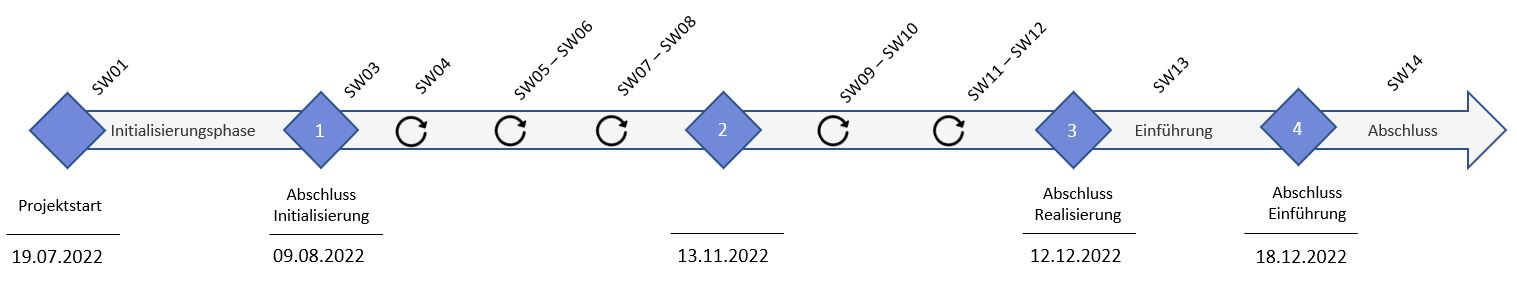
\includegraphics[width=1.3\textwidth]{img/Rahmenplan.jpg}
    \caption{Rahmenplan}
    \label{fig:Rahmenplan}
\end{figure}
\todo{Hinzufügen von Meilenstein am Anfang von Projekt}
\todo{Datum bei Projektstart stimmt nicht}
Es wurde entschieden eine Intialisierungsphase von 3 Wochen zu planen, da die Analyse der bestehenden Software in dieser Phase stattfindet.
Am Schluss bleibt noch eine Woche für die Einführungsphase und das Erstellen der Anleitung.
Für die Realisierungsphase bleiben 9 Wochen Zeit, die in Sprints eingeteilt werden können.
Es verbleibt ein einwöchiger Sprint und 4 reguläre zweiwöchige Sprints.

\subsubsection*{Meilensteine}
Meilensteine erlauben es den Projektfortschritt festzustellen, 
in dem zuvor definierte Projektergebnisse (Artefakte) an einem gewissen Datum vorliegen.\\
Artefakte sind konkrete Dokumente oder Software die vorliegen muss. Zum Beispiel:
\begin{itemize}
    \item Testprotokolle
    \item Prototypen
    \item Software Releases
    \item Sprintplannungen
    \item etc.
\end{itemize}

In SoDa ist es normal, bei jedem Phasenwechsel ein Meilenstein zu definieren und in der Mitte der
Realisierungsphase noch einmal. \autocite{} % PMB Projektplanung p23-25
Nach diesem Vorgehen erhält man 5 Meilensteine für dieses Projekt.

\begin{table}[h]
    \centering
    \begin{tabular}{|l|l|l|}
        \hline
        \rowcolor[gray]{.9} MS & Datum & Artefakte \\
        \hline
        1 & 19.09.2022 & \tabitem Aufgabenstellung \\
        \hline
        2 & 09.10.2022 & \tabitem Architekturdokument \\
         & & \tabitem Analyse \\
         & & \tabitem Testkonzept \\
         & & \tabitem Sprintplannung 1 \\
        \hline
        3 & 13.11.2022 & \tabitem Software-Release 0.5 \\
         & & \tabitem Sprintplannung 4 \\
        \hline
        4 & 12.12.2022 & \tabitem Software-Release 1.0 \\
         & & \tabitem Dokumentation Realisierung \\
        \hline
        5 & 18.12.2022 & \tabitem Bedienungsanleitung \\
        \hline
    \end{tabular}
    \caption{Meilensteine}
    \label{tab: Meilensteine}  
\end{table}

\subsection{Anforderungen}
Aus dem Projektauftrag und aus den Wünschen der Stakeholder werden Anforderungen an das Produkt definiert.
Diese werden für die Realisierungsphase in Epics umgewandelt. 
Die Epics werden im Anschluss in einzelne User Stories aufgeteilt, die dann in den Sprints seperat behandelt und gelöst werden.
\newpage

\subsubsection{Epics}
Für das Projekt werden folgende Epics definiert.

\begin{table}[h]
    \centering
    \begin{tabular}{ | p{1em} | p{35em} | p{2em} |}
        \hline
        \rowcolor[gray]{.9} ID & Beschreibung & Prio \\
        \hline
        1 & Der Nutzer wird beim erstmaligen Betreten des Discord-Servers vom Bot benachrichtigt.
        Dieser gibt ihm Grundlegende Informationen zum Server und dem Authentisierungsprozess.
        Zu diesem Zeitpunkt hat der Student noch keine Berechtigungen auf dem Server Und
        hat nur Zugriff auf den Channel "Help". & A \\
        \hline
        2 & Der Bot soll den Nutzer authentifizieren und mit der Studenten-Rolle versehen können.
        Er kann dabei zwischen den E-Mails von Nicht-Student und Student unterscheiden und auf unvorhergesehene
        Interaktionen, von Seiten des Benutzers, reagieren können. & A \\
        \hline
        3 & Ein Student kann sich beim Bot für ein Modul anmelden. Dieser schaltet den Channel für den Studenten frei,
        so das er darin mit anderen Studierenden kommunizieren kann. Falls das Modul für den Studenten nicht mehr relevant ist,
        kann er es beim Bot wieder abmelden. & A \\
        \hline
        4 & Die Administration des Discord Servers soll einfach neue Modullisten in das System laden können.
        Die neuen oder nicht mehr Verfügbaren Module werden erkannt und entsprechend hinzugefügt oder gelöscht.
        An dem Verhalten des Benutzers soll sich nichts ändern. & A \\
        \hline
        5 & Die Adminsitration kann jedes Semster die neuen Studierenden hinzufügen. 
        Diese werden beim potentiellen Authentifizieren direkt in Ihre zugeteilten Häuser zugewiesen. & A \\
        \hline
        6 & Die Administration von Stair kann über eine zur Verfügung gestellte Schnittstelle Statistiken über 
        den Discord erstellen können. & B \\
        \hline
        7 & Fehlereingaben in den Modulregistrierungschannel oder interne Fehler vom Bot, sollen direkt automatisch 
        an einen hinterlegten Mitarbeiter von Stair gemeldet werden & C \\
        \hline
    \end{tabular}
    \caption{Epics}
    \label{tab: Epics}
\end{table}

\subsubsection{User Stories}


\subsubsection{Sprintplanung}
Some text.
\newpage

\section{Realisierung}

\subsection{Analyse der bestehenden Infrastruktur}
Als erster Schritt wird eine Analyse des bestehenden Bots und seiner Funktion im Discord durchgef\"uhrt.

\subsubsection{Aufbau Discord}
Der Discord Server "Stair" wird von Stair verwaltet und ist ein online Treffpunkt f\"ur alle Studenten des Departements Informatik.
Beim erstmaligen Eintretten in den Server hat man noch keine Berechtigung und es wird deshalb noch nichts, ausser dem Help Channel
angezeigt. Man bekommt vom Bot Stan, beim Eintretten auf den Server, eine Nachricht mit einer Anleitung. Darin ist beschrieben, wie
man sich authentifizieren kann. Bei der Authentifizierung wird vom Bot geschaut ob es sich um eine Studenten E-Mail Adresse handelt.
Wenn dem so ist, schickt der Bot einen 6-stelligen Random Code, den der Benutzer im Discord dem Bot zur\"uckschreiben muss.

Hat dieser Prozess funktioniert, ist man "eingeloggt" und bekommt vom Bot die Rolle Student zugeteilt. Damit hat man Zugriff auf 
die verschiedenen Grundchannels, wie Gaming, Administration, General, Studying, etc.
In diesen Channels kann man sich mit seinen Mitstudierenden Sprachlich oder per Text \"uber alle Themen austauschen.
\newline

Der Stair Discord-Server bietet auch Informationen und Unterst\"utzung f\"ur alle Module an. Dabei hat jedes Modul einen eigenen Channel.
Dort k\"onnen sich Studierende gezielt \"uber ein Modul austauschen, Fragen stellen oder Informationen mitteilen.
Am Anfang wird gar nichts angezeigt. Man muss sich spezifisch f\"ur die Module registrieren um diese angezeigt zu bekommen. Dies verhindert

\begin{enumerate}
    \item dass man unn\"otig Benachrichtigungen von Channels bekommt, die einen nicht interessieren.
    \item dass sein Discord nicht \"uberf\"ullt wird mit 400 Modul-Channels.
\end{enumerate}

Die Commands \textit{show <module>} und \textit{hide <module>} erlauben es, den Channel hinzuzuf\"ugen oder zu entfernen. 
\newline

Neu gibt es auch das Konzept von verschiedenen H\"ausern bei Stair. Jeder Student wird dabei einem Haus zugeteilt. Die Zuteilung l\"auft
dabei \"uber das Sekretariat der Hochschule. Es wird geschaut, dass in jedem Studiengang in jedem Startsemester, die Studenten gleichm\"assig
auf die H\"auser verteilt werden.
Es gibt die H\"auser Blue, Purple, Red, Orange, Yellow und Grey. \"uber das Semester hinweg organisiert Stair verschiedene Events, bei denen
man Punkte f\"ur sein Haus sammeln kann. Am Ende jedes Jahres, also Ende Fr\"uhlingssemster, wird das Haus, welches am meisten Punkte 
gesammelt hat, als Gewinner gelobt.

Der Discord-Server bietet die Platform um sein Haus zu mobilisieren oder die neuesten Ergebnisse den Studenten zu verk\"unden.
Pro Haus gibt einen Channel. Momentan werden die Studenten noch manuell zu ihren zugeh\"origen Channels hinzugef\"ugt.
\newline
\newline
\todo{Bild von Discord und Channels anzeigen}

\subsubsection*{Ablauf Athentifizierung}
\todo{Nicolas}
\todo{Bild Ablaufdiagramm Authentifizierung}


\subsubsection*{Ablauf Modul-Channel Einschreibung}
\todo{Bild Ablaufdiagramm Modul}


\subsubsection{Funktionsweise Bot}
Der Bot ist mit der Programmiersprache C\# und dem .NET Framework geschrieben. 
In der folgenden Tabelle ist eine \"Ubersicht der benutzen IDE, ihrer Spezifizierung und den eingesetzten Libraries.
\todo{Tabelle mit Spezifikationen vom System. (Versionen, Libraries)}
\newline


Das Programm, welches den Bot zur Verfügung stellt, ist nicht gross. Es beinhaltet im Groben einen Client Socket der 
Events on Discord abfängt und einer E-Mail Klasse, die E-Mails an den Benutzer versenden kann.
Das Programm ist in zwei Packages aufgeteilt.

\begin{itemize}
    \item StanBot.Core
    \item StanBot.Service
\end{itemize}

\todo{Bild Klassendiagramm Bot}

\subsubsection{Ausführung Bot}

Der Bot läuft auf einem Windows Server \#\#\#\# auf der Enterprise Lab Umgebung der HSLU. Die Konfiguration entspricht der eines
Windows Services und läuft dementsprechend durchgehend.
\newline
\todo{Bild Service Konfiguration}
\newline


\subsubsection{Geplante Änderungen}
\todo{Yannis}
Wechsel auf Linux Server, warum


Entscheid neuer Bot schreiben, mit neuen Libraries.


Entscheid von Login mittels E-Mail, nicht über Switch Account.


Entscheid wechsel auf Community server


Entscheid Anbindung an Datenbank
- Einfachere Verwaltung von Studenten und Modulen
- Einfachere Kontrolle und Steuerung von Stair
- Erweiterbarkeit und Weeiterentwicklung
- Anbindung von anderen Tools/Programmen an Datenbank (Statistik/Zukunft)

Entscheid schreiben eines eigenen Bots
- Bestehender Bot
- Datenschutz
- Kontrolle und Handlungsspielraum
- Statistiken
- Keine ungewollten Features

\subsection{Sprint 1}

\newpage
\section{Evaluation und Validation}

\todo{schreiben}

\section{Ausblick}

\todo{schreiben}

\newpage

\section{Anh\"ange}

\todo{schreiben}

\section{Glossar}

% https://blog.aristolo.com/de/definition-begriffe-bachelorarbeit-masterarbeit-dissertation/
\todo{schreiben}

\section{Abbildungsverzeichnis}
\listoffigures

\section{Tabellenverzeichnis}
\listoftables

\section{Literaturverzeichnis}
\printbibliography

\end{document}
